% \todo{Rewrite Introduction to match the conclusion and abstract}
\chapter{Introduction}\label{chap:Introduction}
The demand for power to run computational tasks is accelerating. To overcome the increasing complexity, the transistors which do the heavy lifting of storing and computing the singular 0's and 1's, have been stacked closer and closer. Now, they span only few nanometer, a size where they are susceptible to quantum effects, creating new challenges. \cite{morton_embracing_2011}. The same quantum effects also prove a hope, since they can be utilized in a new form of computing on different devices, quantum computers. 

By considering quantum bits with the ability of being in a super position of 0 and 1, some large problems can be formulated compactly and run efficiently \cite{preskill_quantum_2018}. That is, if one has a working quantum computer. Many different implementations of quantum computers are well on their way, taking on many forms. Some promising candidates are  singular atoms trapped in electric fields and controlled by lasers \cite{brown_co-designing_2016}, single photons capable of storing quantum information \cite{obrien_optical_2007}, or superconducting circuits which are controlled by microwave pulses at temperatures just above the absolute zero \cite{krantz_quantum_2019}. The latter will be the focus of this thesis. 

Superconducting qubits are rapidly developing and has seen multiple big accomplishments in the last few decades: the design and fabrication of superconducting circuits capable of processing quantum information \cite{koch_charge_2007, manucharyan_fluxonium_2009}, microwave pulses that can control and read it out with high precision \cite{motzoi_simple_2009, READOUT} and schemes to entangle qubits with their neighbors \cite{yan_tunable_2018}. Recent progress has improved the ability to do operations on a single superconducting qubits \cite{barends_superconducting_2014} and multi qubit gates have surpassed the 99.9 \% fidelity mark\cite{ding_high-fidelity_2023}. Improvements have also been made for qubit initialization and readout\cite{walter_rapid_2017, swiadek_enhancing_2023}, but this is still a challenge. The State Preparation and Measurement errors (SPAM) are often listed under the same acronym together because they are inseparable in a quantum algorithm \cite{SPAM}. In this thesis, we will instead take address the physics behind the measurement process allowing us to build a model of our system in simulation, where we investigate the effect physical parameters have on the SPAM errors. 


% State preparation and measurement errors (or SPAM for short) are difficult to separate and is limiting the ability to run larger quantum circuits. By first understanding the physics of a superconducting qubit readout, we will in this thesis built models allowing us to dive deep in how different physical parameters contribute to the SPAM errors.



% \newpage
\section{Outline of Thesis}
The thesis is built up in the following way. The first few chapter will mainly be theoretical. In the rest of chapter \ref{chap:Introduction}, we will cover some fundamentals of quantum mechanics and in chapter \ref{chap:cQED} we will focus in particular on the theory of circuit Quantum Electrodynamics (cQED). Chapter \ref{chap:computations_and_readout} will go into more depth of how the qubit can be connected with control hardware to allow control and readout of the qubit. Furthermore, we will investigate how interactions with the environment affects our qubit. This is done by discussing open quantum systems in chapter \ref{chap:open_quantum_systems} and weak continuous measurements in chapter \ref{chap:measurements}.

The second half of the thesis will focus on readout in experiment and our efforts to recreate it in simulation. We will in chapter \ref{chap:readout} present the experiment to investigate the performance of readout in our system. In chapter \ref{chap:calibration} we will calibrate it to determine the necessary parameters for simulating it. The simulation is created and discussed in \ref{chap:model}. Finally, we will in chapter \ref{chap:budget} use our model to investigate how different parameters contribute the readout and state preparation infidelity in our system by changing them in our model.  



% \todo{Update the outline and write coherently}
% \begin{itemize}
%     \item In the first section, we will review the circuit quantum electrodynamics (cQED) which gives rise to the potentials we base our qubit and readout resonator on.
%     \item We will go into depth of how this system can be viewed in the light of the parameters and limits we impose on the system.
%     \item The thesis will the cover, how our system interacts with the environment. This will give rise to the Lindblad Master Equation and a discussion of decoherence of our quantum system. 
%     \item Then we will go through how the system is measured. For this we will need to go through the (1) the stochastic master equation which arises in continuous measurements, (2) the microwave field which we will see in the drive line and in the resonator, (3) the amplification chain that leads the resonator signal at 10 mK into the lab and (4) how the signal can be read out by either a homodyne or heterodyne measurement.
%     \item A section focusing on how the IQ plane of the resonator can be used to calibrate different errors. We will hopefully be able to separate State Preparation and Measurement errors using the physics happening in the two.
%     \item A part covering the simulations we can put together from the above. How can we use this to best distiguish the $\ket{0}$ and $\ket{1}$ state. 
%     \item Hopefully, this can be followed by a section where we fit the master equation or stochastic master equation to calibrate hamiltonian of the system while measured.
% \end{itemize}

\section{Qubits}
Improving classical computer hardware can take many shapes: more processing power, bigger memory size, or faster data transfers. Ultimately, these improvements increase our capability of storing, messaging, or manipulating single entities, bits. Bits the smallest piece of information corresponding to an on/off switch. Often they are represented with binary numbers, such that "1" is on and "0" is off. Combining billions or even trillions of bits, we can store data, media or even programs.

While most everyday computing tasks can easily be done using classical computers, some problems scale exponentially and unforgivably when the size of the problem is increased. Among these problems, we find prime factorization and simulation of quantum mechanical systems, a challenge which will hunt us through this thesis. Instead of building classical computers of exponentially increasing size, quantum mechanics provides a hope to solve these problems by replacing the bit with the quantum bit (qubit). The qubit is not bound by the discreteness of the classical bit but can be in a superposition of "0" and "1" at the same time \cite{krantz_week_2019}.

\subsection{A Quantum Mechanical State}
In quantum mechanics, the properties of our system can be of continuous like the position of a particle or discrete like the spin of an electron, pointing either up or down. When considering a quantum mechanical object, all possible physical configurations span a Hilbert Space of finite or infinite dimensions. A set of configurations which completely describes all information one could measure of an object is an element in the Hilbert space and is called a quantum mechanical state. Mathematically, we represent it with a ket: $\ket{\psi}$ where $\psi$ is just a label \cite{sakurai_modern_2021}.

The observable information about the state of the system can be found by applying operators to it. Applying an operator is represented as multiplication from the left: $A\ket{\psi}$, which illustrates the linearity of quantum mechanics. Of special interest are eigenstates to an operator, which are states satisfying $A\ket{a} = a \ket{a}$, where $a$ is the eigenvalue and $\ket{a}$ is the eigenstate. Most importantly is perhaps the energy of the system and the corresponding energy eigenstates. These are states associated with Hamiltonian operator which like in classical mechanics generates the equation of motions in quantum mechanics \cite{sakurai_modern_2021}.

\subsection{The Two Level System}\label{sec:tls}
To create a qubit, one needs a quantum mechanical system with two levels. There are multiple ways of achieving this. A straightforward approach is by using an observable in a 2-dimensional Hilbert space like the spin of an electron.  

Another approach is to limit ourselves to only a subspace of a larger Hilbert space. If the quantum mechanical states is connected to an environment, they are subject to Boltzmann statistics \footnote{That is the relative probability of finding a qubit in two different states (say $\ket{1}$ and $\ket{0}$) can be found as the fraction between their Boltzmann factor: $e^{-E_1 / k_b  T} / e^{- E_0 / k_b  T}$.}. At low enough temperatures where the energy different is much larger than the temperature $\Delta E \gg k_b T$, the system will occupy the ground state unless we change it. By limiting our operation to the subspace of "0" and "1", we will effectively have a qubit \cite{boltzmann}. 

After choosing a two level system, the states of the system can be described as $\ket{0}, \ket{1}$ and can be combined to construct superpositional states:
\begin{equation}
    \ket{\psi} = a \ket{0} + b \ket{1}
\end{equation}
where $a$ and $b$ are complex numbers and $|a|^2, |b|^2$ are the respective probabilities that the state will collapse to either $\ket{0}$ or $\ket{1}$ if measured. Since the probabilities must sum to one, we have normalization constraint. We are also allowed to freely choose a global phase since only phase differences have physical meaning\cite{}. These constraints allow us to write a general state of the two level system:
\begin{equation}\label{eq:general_2_state}
    \ket{\psi} = \cos (\theta / 2) \ket{0} + e^{i\phi}\sin(\theta / 2)\ket{1}
\end{equation}
where our description have two angles $\theta$ and $\phi$ which determine the relative occupation in these two states and a phase between them. With these two angles, the state of a qubit can be visualized geometrically \cite{krantz_quantum_2019}.

\subsection{The Bloch Sphere}
A perfect place to visualize two angles $\theta$ and $\phi$ and a length of 1 is a point on the unit sphere. The depiction of a qubit state on a sphere is called a Bloch Sphere and an example can be seen in \ref{fig:bloch_sphere}. On the Bloch Sphere, the state $\ket{0}$ will be on the north (positive) pole along the z-axis and $\ket{1}$ at the south pole (negative). With this mapping the projection of the state vector unto the z-axis gives the probabilities of finding $\ket{0}$ or $\ket{1}$ respectively and the phase difference is mapped unto the x-y plane  \cite{krantz_week_2019}.

\begin{marginfigure}[- 7 cm]
    \centering
    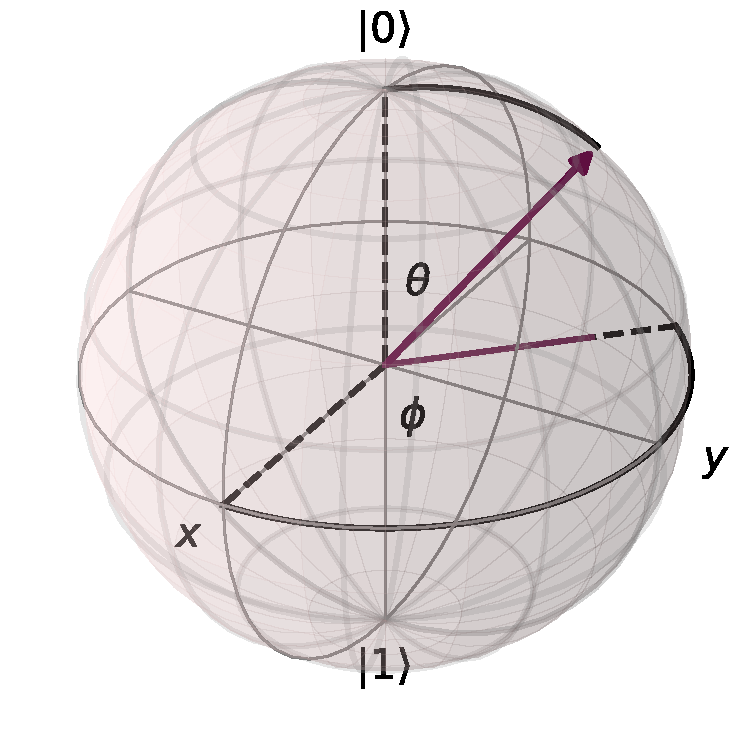
\includegraphics[]{Figs/Theory/bloch_sphere.pdf}
    \caption{Representation of a qubit state on the Bloch sphere. The angles $\phi$ and $\theta$ are displayed along with the projection onto the x-y plane.}
    \label{fig:bloch_sphere}
\end{marginfigure}

% \section{Time Evolution of a Quantum System}
% As a physics student, one is often met early in ones career by Newtons second law, stating that acceleration equals force times mass $\Vec{F} = m \Vec{a}$. Knowing the force asserted on an object thus gives the equations of motion. Often it is however more beneficial to represent the equations of motions in the Hamiltonian formalism, where one can derive the equations of motion by the energy of the system (the Hamiltonian). The equation of motions are now given by a coordinate and the canonical momentum to that coordinate. 

% In this formalism the time dependence of the coordinates $q$ and canonical momentum $p$ is given by\footnote{The canonical momentum is found from the Lagrangian which is related to the Hamiltonian by a Legendre transformation} :

% \begin{align}
%     \dot{p} = - \pfrac{}{q} &H(p, q) \\
%     \dot{q} = \pfrac{}{p} &H(p, q)
% \end{align}

% Or for a general function of a set of coordinates and the set of canonical momenta $f(\{q_i\}, \{p_i\}, t)$, we can represent the time-dependence using Poisson brackets: \cite{Fetter_continous_mechanics}
% \marginnote{A Poisson bracket refers to a specific combination of differentials. With $\{F, G\} = \sum_i \left(\pfrac{F}{q_i} \pfrac{G}{p_i} - \pfrac{F}{p_i} \pfrac{G}{q_i} \right)$} 

% \begin{equation}
%     \dot{f} = -\{H, f\} + \pfrac{}{t} f 
% \end{equation}

% \paragraph{Going Quantum - }
% From the Hamiltonian formalism the switch to quantum mechanics is significantly shorter. By first introducing the commutator between two operators: \todo{Introduce operators above with operators and uncertainty principle}
% \begin{equation}
%     \comm{A}{B} = AB - BA
% \end{equation}

% Now making the mapping from Poisson brackets to commutators with the appropiate prefactor, we find the correspondence principle:

% \begin{equation}
%     \{A, B\} \to \frac{\hbar}{i} \comm{A}{B}
% \end{equation}

% Such that the time dependence of an operator is given by:
% \begin{equation}
%     \dot{A} = \frac{i}{\hbar} \comm{H}{A} + \pfrac{}{t} A
% \end{equation}

% \textbf{Get to Schödingers Equation here}

% \textbf{Maybe introduce like this instead} \\ \noindent
\section{Time Evolution of a Quantum System}\label{sec:scroedinger}
Let us now take a look at the dynamics of a quantum system. A process which transforms a state into another must leave the inner product unchanged to keep the normalization. By applying unitary transformation this is guaranteed\footnote{For unitary transformations we have: $\unitary^{-1} = \unitary^\dagger$ or equally $\unitary^\dagger\unitary = \identity$}. Quantum dynamics can then be described by a unitary transformation taking a state at some time $t = t_0$ into a the state at a later time $t = t_0 + \Delta t$. At the later time the inner product should be conserved:
\begin{equation}
    \braket{\psi; t_0}{\psi; t_0} = \braket{\psi; t_0 .. \Delta t}{\psi; t_0 .. \Delta t} = \mel{\psi; t_0}{\unitary^\dagger (\Delta t) \unitary(\Delta t)}{\psi; t_0} 
\end{equation}
which is satisfied since $\unitary$ is unitary. An additional requirement is that the transformation should reduce to identity if no time has passed: $\unitary(\Delta t) \to \identity$ when $\Delta t \to 0$. Expanding the transformation in the infinitesimal timestep, $dt$, the unitary transformation is described by:
\begin{equation}\label{eq:infinitesimal_time_evolution}
    \unitary(dt) = \identity - i \Omega dt
\end{equation}
Where $\Omega$ is a hermitian operator with units of frequency\footnote{To see why this keeps the normalization, we write $\unitary^\dagger(dt)\unitary(dt) = (\identity + i \Omega dt)(\identity - i \Omega dt) = \identity + dt^2 \Omega^2$ which goes to identity in the limit of $dt \to 0$ as the $dt^2$ term vanishes.}. 
The actual operator is proportional to the Hamiltonian operator and is given by : $\Omega = \frac{H}{\hbar}$. From eq. \ref{eq:infinitesimal_time_evolution} and by defining $d\ket{\psi; t} = \ket{\psi; t..dt} - \ket{\psi; t} $ we find a differential equation for state evolution:
\begin{align}
    \ket{\psi; t..dt} &= \unitary(dt) \ket{\psi; t} = \left(\identity - i \frac{H}{\hbar}   dt\right) \ket{\psi} \\
    \ket{\psi; t..dt} - \ket{\psi; t} &= i \frac{H}{\hbar}   dt \ket{\psi} \\
    i \hbar \frac{d}{dt}\ket{\psi} &=  H \ket{\psi}
\end{align}
This is known as the Schrödinger's equation and governs unitary time evolution of quantum mechanical system given that it is closed from the environment and is not measured \cite{sakurai_modern_2021}. We will return to these two assumptions and relax them later.

Depending on the Hamiltonian, we can express the time-evolution operator. If the Hamiltonian is independent of time, we can solve the equation above to find:
\begin{equation}
    \unitary(\Delta t) = e^{-iH\Delta t/\hbar}
\end{equation}
which entirely removes the time-dependence from the state such that $\ket{\psi; t} = \unitary(t)\ket{\psi; t = 0}$. If on the contrary, the Hamiltonian is dependent on time and commutes at different times, we can write it as:
\begin{equation}
    \unitary(\Delta t)\ket{\psi; t_0} = \exp\left(-\frac{i}{\hbar}\int_{t_0}^{t_0 + \Delta t} dt H(t)\right)\ket{\psi; t_0}
\end{equation}
If the Hamiltonian at different times do not commute with itself, one could introduce the Dyson series\cite{sakurai_modern_2021}. Another approach is to solve the differential equation numerically.

\subsection{Numerical Implementations}\label{sec:numerical_implementations}
Schrödinger's Equation gives a simple linear relation between the time derivative of a state and the Hamiltonian. If we can represent the states as vectors and the Hamiltonian as matrix, we can naively solve the differential equation by doing finite size step. With $dt\to\Delta t$ The state at $t+\Delta$ will approximately be:
\begin{equation}
    \Vec{\psi}(t + \Delta t) =  \Vec{\psi}(t) - \frac{i\Delta t}{\hbar}\boldsymbol{H} \Vec{\psi}(t)
\end{equation}
Of course this is a crude approximation which improves as $\Delta t$ is reduced and the equation is repeated more. While this method, known as Euler integration \cite{euler}, is simple to implement, it quickly loses precision if the time steps become large (see example in figure \ref{fig:euler_integration}). Instead of improving accuracy by increasing the amount of steps, we instead look at a more sophisticated algorithm.
\begin{marginfigure}
    \centering
    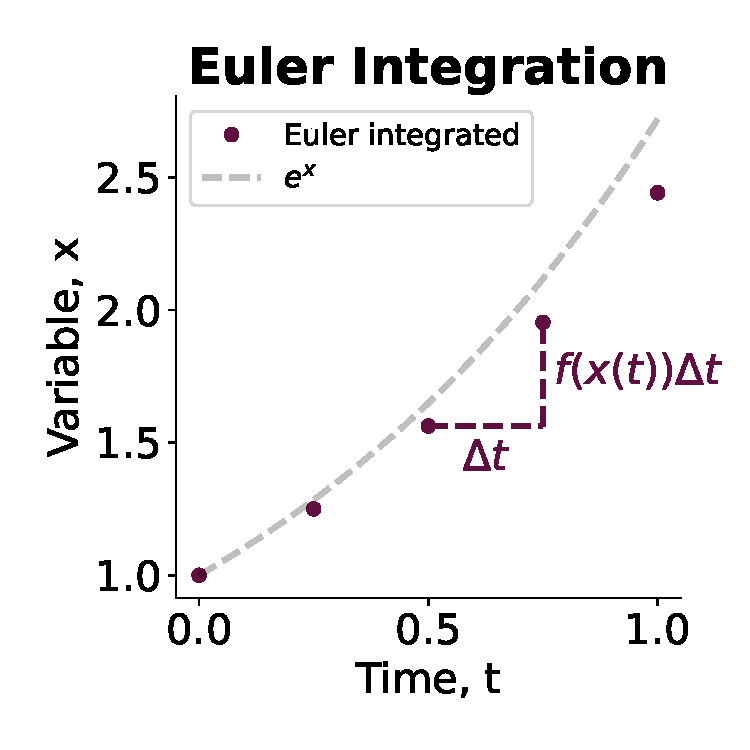
\includegraphics[]{Figs/Theory/euler_integration.pdf}
    \caption{Example of Euler integration $x'(t) = x$}
    \label{fig:euler_integration}
\end{marginfigure}


In this thesis, integration will primarily be performed using the Qutip Library\cite{johansson_qutip_2012}, where the Schrödinger equation is integrated by the Adams method. In this method we the last $n$ points in order to  approximate the higher order differentials of the function. If we have a differential equation:
\begin{equation}
    y'(t) = f(y(t))
\end{equation}
We can approximate the point $y(t+\Delta t)$ by a Taylor expanding around $t$:
\begin{equation}
    y(t) + \Delta t y'(t) + \frac12 \Delta t^2 y''(t) + \frac{1}{3!} \Delta t^3 y'''(t)\dots 
\end{equation}
The idea in the Adams algorithm is to approximate the differential up to order $n$ by using finite difference methods. The first and second order derivative can then be approximated by:
\begin{equation}
    y'(t) = f(t), \quad y''(t) = \frac{f(y(t)) - f(y(t - \Delta t))}{\Delta t} 
\end{equation}
And the third order differential by:
\begin{equation}
    y'''(t) = \frac{y''(t) - y''(t-\Delta t)}{\Delta t} = \frac{f(y(t)) - f(2y(t-\Delta t)) + f(y(t-2\Delta t))}{\Delta t^2}
\end{equation}
\begin{marginfigure}
    \centering
    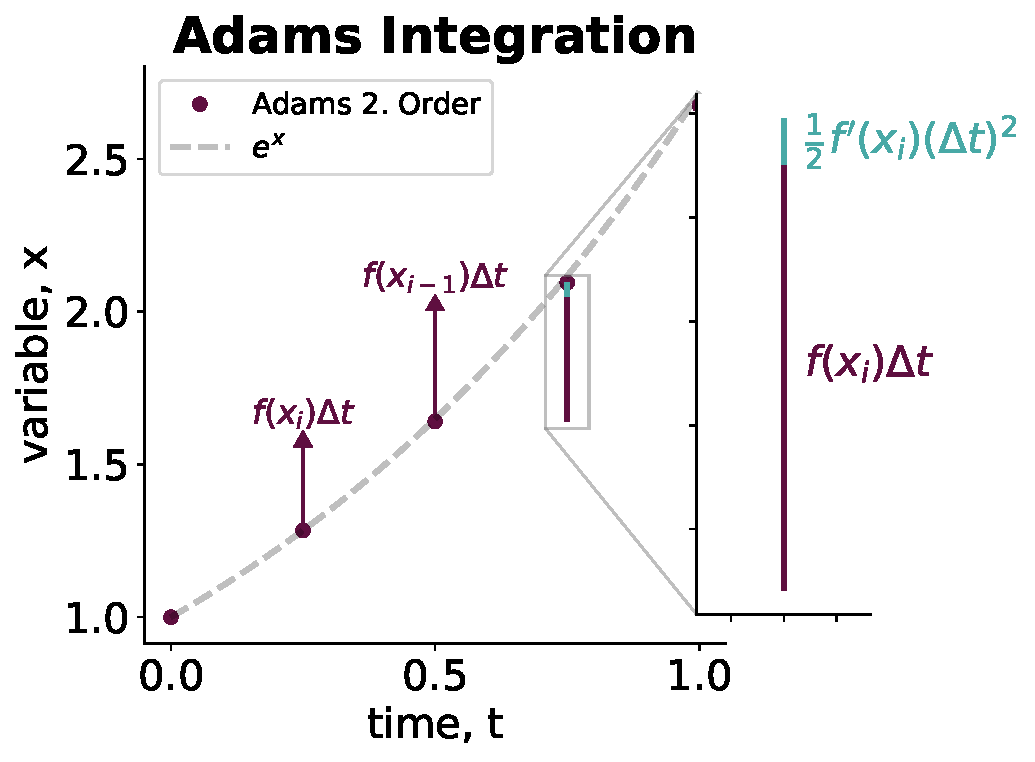
\includegraphics[width = 1.2 \linewidth]{Figs/Theory/adams_intergation.pdf}
    \caption{How the Adams algorithm works. Here the second order derivative is found by the finite difference method to be $f'(x_i) = (f(x_i) - f(x_{i-1}))/\Delta t$}
    \label{fig:Adams integration}
\end{marginfigure}
and on wards. A visualization of the second order method can be seen in figure \ref{fig:Adams integration}. The computation of the Adams algorithm is more precise since it considers higher order terms and it runs fast since it reuses the old calculations. 

One challenge is that the algorithm requires $n$ points to get started. Before the $n$ points, we can assume no higher order differentials, such that we effectively perform Euler integration for the first step and a second order Adams for the second and so on. Alternatively, we can use another algorithm which moves forward in time to approximate the higher order differentials. An example of such an algorithms is the Runge-Kutta method, which is used in most modern solvers for ordinary differential equations \cite{butcher_numerical_2000}. 

% \todo{Check with source here: \url{https://link.springer.com/book/10.1007/978-3-540-78862-1} should be accessible within KU }
% \textit{The Runge-Kutta method goes forward in time to find intermediate time steps, where the differential equation again is evaluated. When summing the different paths, the errors cancel out up the order $n$, where $n$ is the amount of intermediate steps. To second order, the Runge-Kutta algorithm calculates half a time step: $k_1 = \Delta t / 2 \psi$ and averages the slope of the slope of the given point and the next. 
% }
% $ takes $\Vec{\psi_i} = \Vec{\psi_{i-1}} + k_1 + \mathcal{O}(\Delta t^3)$. To higher orders this lets us suppress the error for the first few steps using multiple steps with the Runge-Kutte method and when we have the first $n$ values, we can switch to the Adams method to improve speed while keeping the error small. \todo{Same source as above? } 
% \todo{Write this properly}
% \paragraph{Adams method} includes the values calculated in the last few steps to determine a polynomial expansion. This does not require to calculate as many points as the Runge-Kutta and comes with a high precision as well. Requires a few points to start, but one could use Runge-Kutta to find the first few points or run the algorithm backwards in time. 


% The Adam package is also the one used in the Qutip package which is used for this thesis. Here the algorithm is run to 12 order with a set error tolerance and the possibility to adapt and take multiple steps between the desired resolution.

\section{Computational Framework of the Thesis}
\begin{figure}[h]
    \centering
    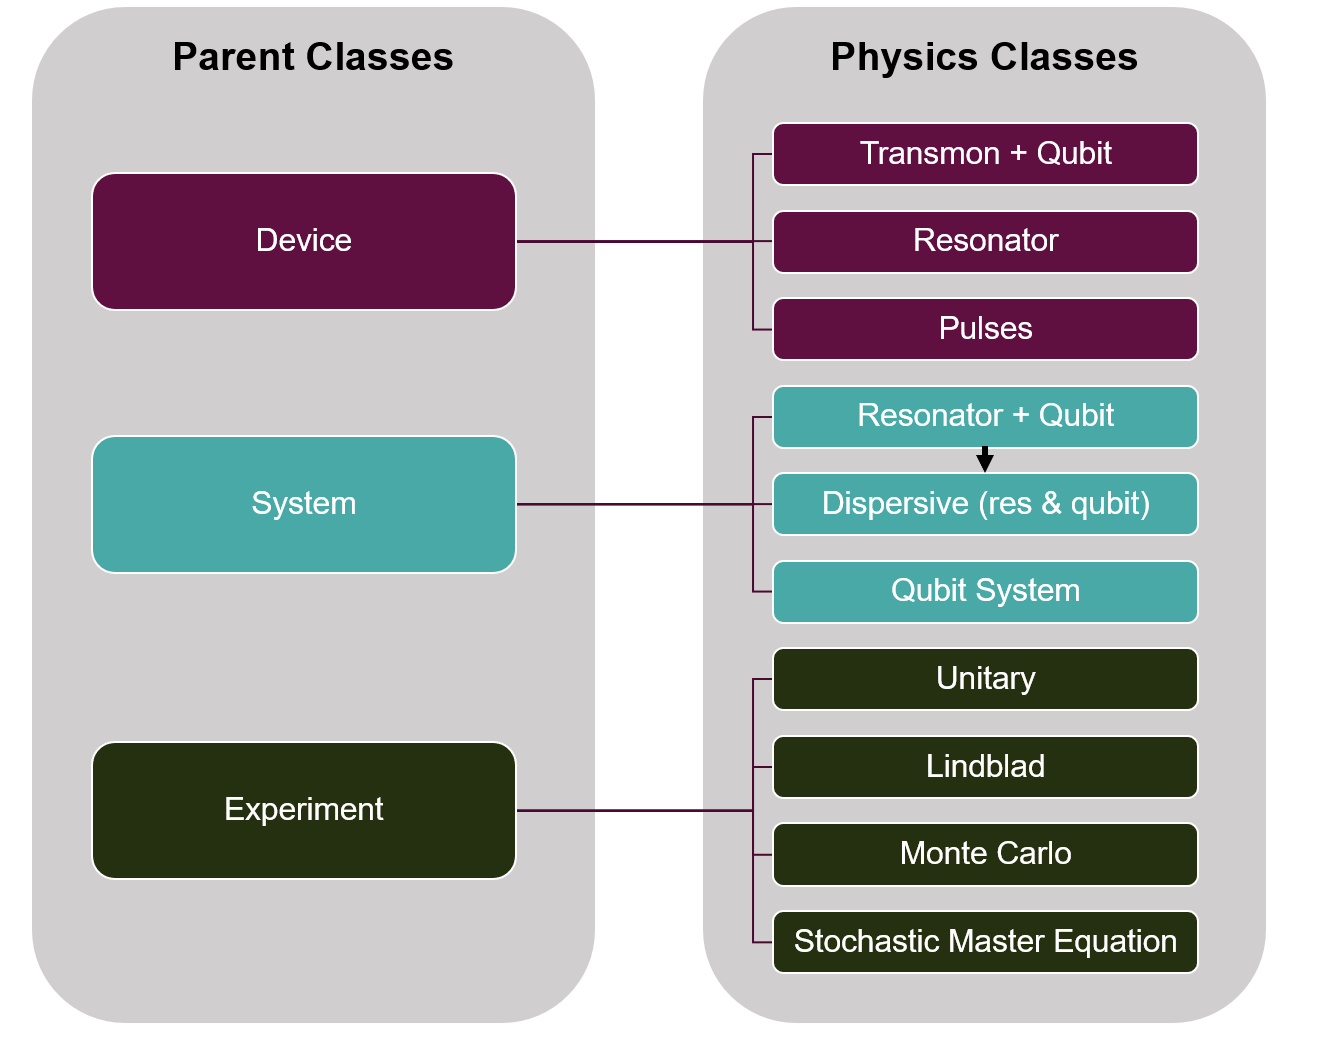
\includegraphics[width = 1.0 \textwidth]{Figs/Sections/Introduction/module_v2.png}
    \caption{Module structure divided into the Parent Classes maintainining parameters and sweeping and the Phyics classes which serves as containers for Hamiltonian, dissipation operators or simulation schemes.}
    \label{fig:module_overview}
\end{figure}
It is by no means a new idea to solve quantum mechanical problems by numerical simulations, so multiple well-optimized and versatile libraries exist. In this thesis, we base most of the calculations on the integration methods present in the Qutip Library \cite{johansson_qutip_2012}. To make faster progress and hopefully contribute to the software in the laboratory, a module to make numerical superconducting qubit experiments was developed during this project. The package is a wrapper around the Qutip Library, but eases the setup of calculating Hamiltonians in superconducting systems, running simulations and managing data. The documentation for the module QuantumDeviceSimulation can be found in appendix \ref{chap:code_documentation}.

An overview of the module is shown in figure \ref{fig:module_overview}. In general, it is built in three main parts:
\begin{itemize}
    \item \textbf{Devices} are the physical devices placed in the system. This includes different qubits, resonators and pulses.
    \item \textbf{Systems} are combinations of devices along with descriptions of how they interact.
    \item \textbf{Experiments} are organizing the different sweeps of parameters and applying the proper integration technique. 
\end{itemize}